% Name: Simple flowchart
% Description: Start, one step, one decision, and stop, with default styling to build on.
% Tags: flowchart, process, decision

\usetikzlibrary{shapes.geometric, arrows.meta, positioning}

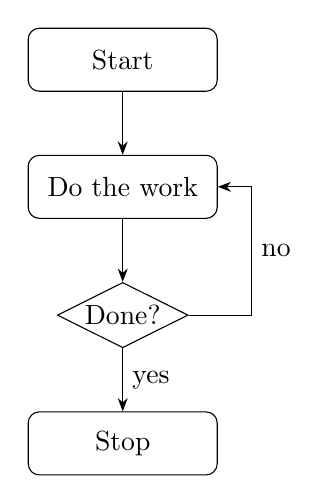
\begin{tikzpicture}[
  node distance=8mm,
  box/.style={draw, rounded corners, minimum width=24mm, minimum height=8mm},
  choice/.style={draw, diamond, aspect=2, inner sep=1pt},
  every edge/.style={draw, -{Stealth}},
]
  \node[box] (start) {Start};
  \node[box, below=of start] (step) {Do the work};
  \node[choice, below=of step] (check) {Done?};
  \node[box, below=of check] (stop) {Stop};

  \path (start) edge (step)
        (step) edge (check)
        (check) edge node[right] {yes} (stop);
  \draw[-{Stealth}] (check.east) -- ++(8mm,0) |- node[pos=0.25, right] {no} (step.east);
\end{tikzpicture}
